% Formatering av framsida

\begin{titlepage}

\includegraphics[height=2.0cm]{mah_logo.eps}
\begin{center}
  
% Upper part of the page. The '~' is needed because \\
% only works if a paragraph has started.
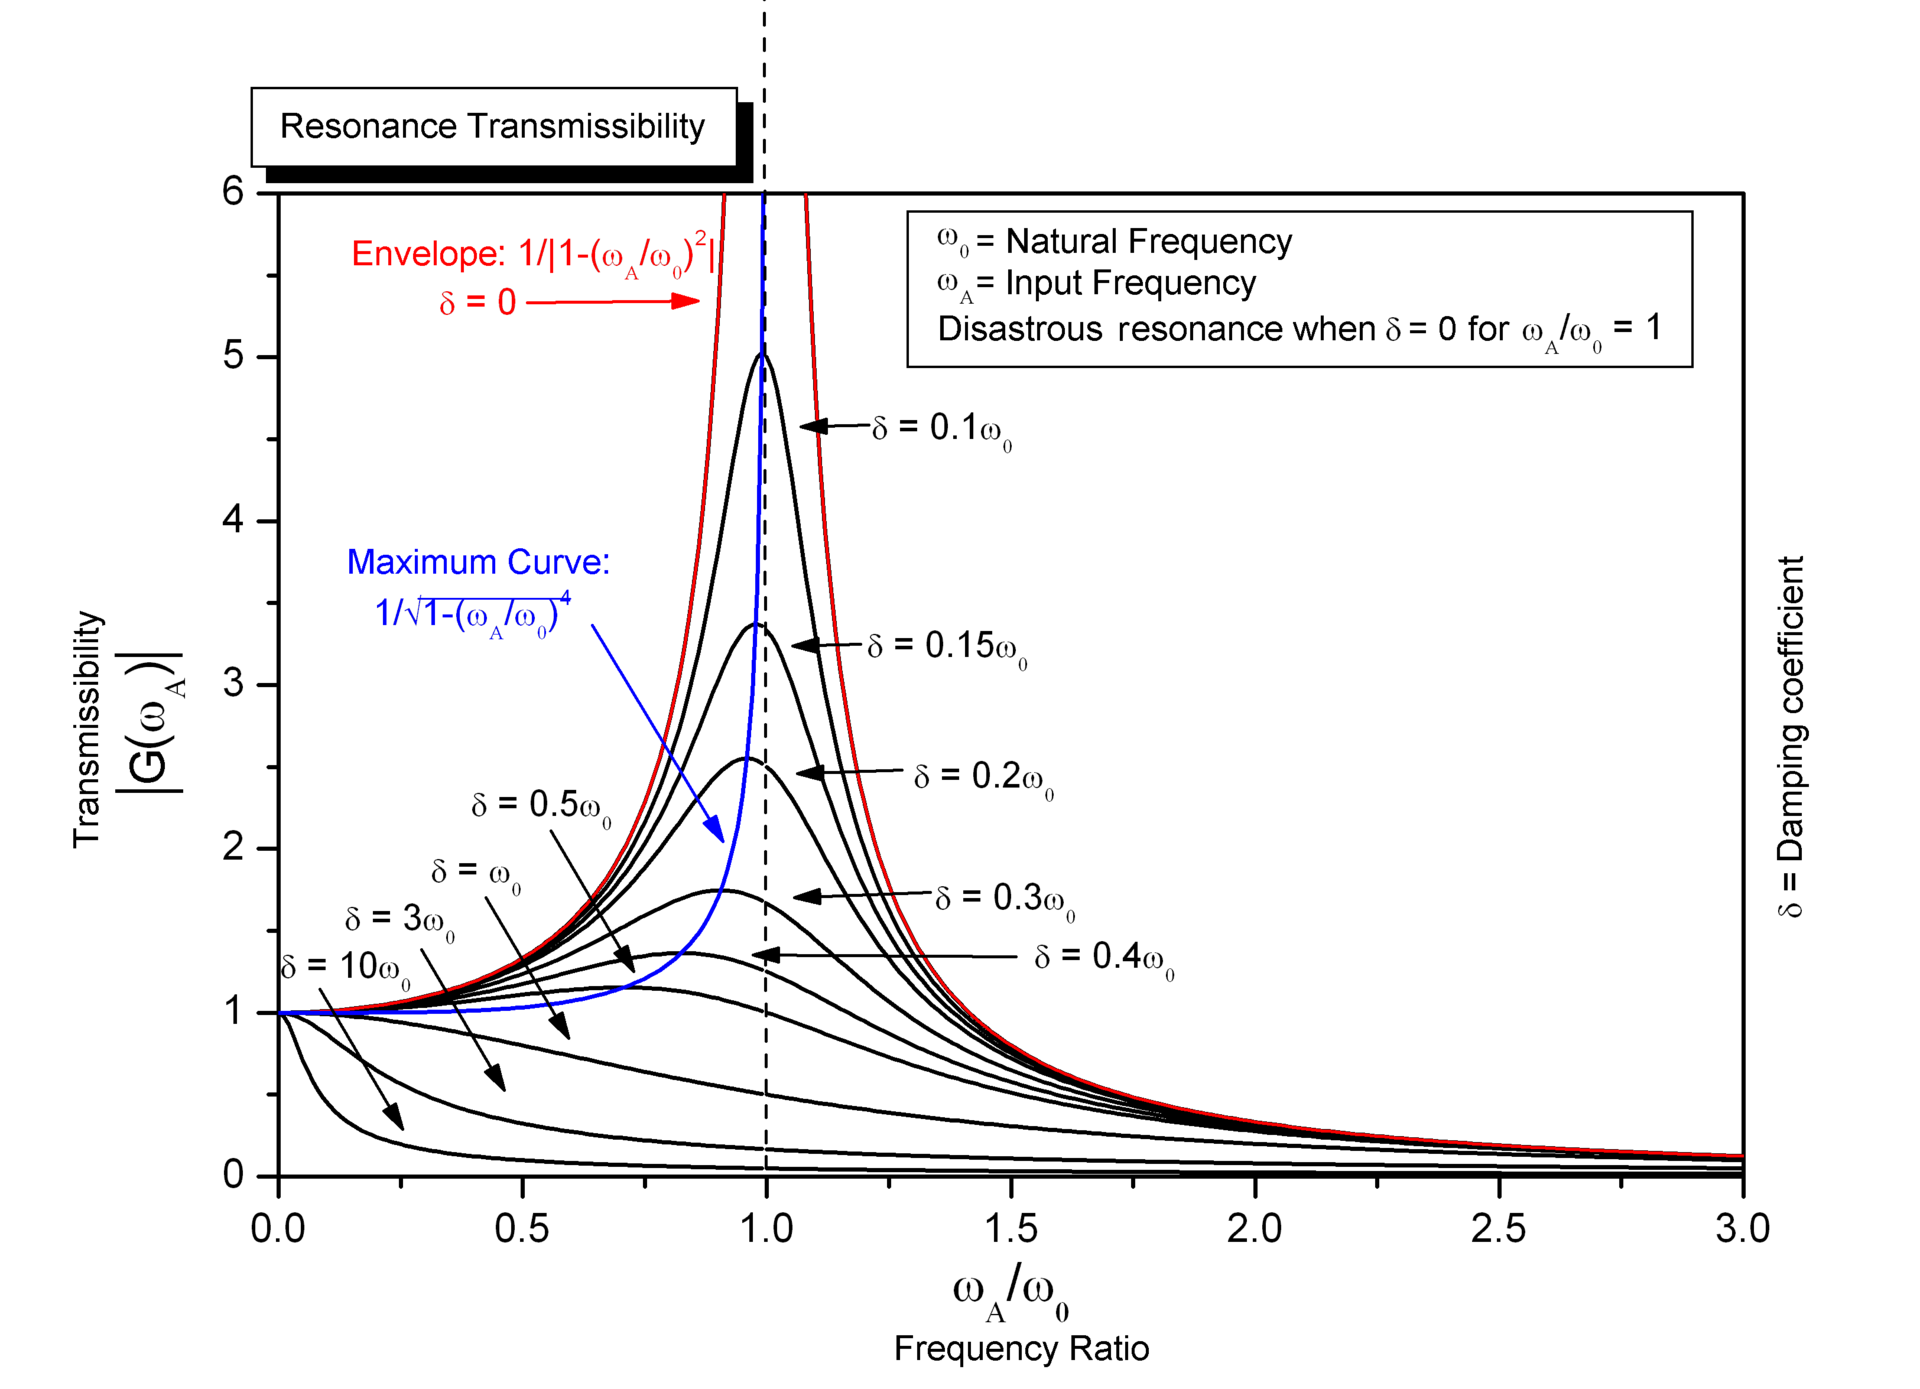
\includegraphics[width=0.15\textwidth]{./fig1.png}~\\[1cm]

{\LARGE Arbetsuppgift \#:\\ [0.2cm]}

{\Large eventuell undertitel\\ [1.0cm]}

\begin{flushright}
Modeller och verklighet, Datateknik, HT15 \\
\end{flushright}
\vfill
\begin{flushleft}
  {\bf Grupp:} \#\# \\
  {\bf Namn:} Förnamn Efternamn \\
  {\bf Namn:} Förnamn Efternamn \\
  {\bf Namn:} Förnamn Efternamn \\
  {\bf Namn:} Förnamn Efternamn \\
  ~\\
  Datum för inlämning: ÅÅMMDD \\
  ~\\
  Status:\\
  \vspace{5mm}

  \begin{tikzpicture}[line cap=round,line join=round,>=triangle 45,x=1.0mm,y=1.0mm]
\draw (-5,10)-- (0,10);
\draw (0,10)-- (0,5);
\draw (0,5)-- (-5,5);
\draw (-5,5)-- (-5,10);
\draw (2,10) node[anchor=north west] {Ny inlämning senast:};
\draw [dotted] (40,5)-- (100,5);
\end{tikzpicture}\\

  \begin{tikzpicture}[line cap=round,line join=round,>=triangle 45,x=1.0mm,y=1.0mm]
\draw (-5,10)-- (0,10);
\draw (0,10)-- (0,5);
\draw (0,5)-- (-5,5);
\draw (-5,5)-- (-5,10);
\draw (2,10) node[anchor=north west] {Godkänd med betyg:};
\draw (40,10)-- (50,10);
\draw (50,10)-- (50,5);
\draw (50,5)-- (40,5);
\draw (40,5)-- (40,10);
\end{tikzpicture}\\

  \begin{tikzpicture}[line cap=round,line join=round,>=triangle 45,x=1.0mm,y=1.0mm]
    \draw (-5,10)-- (0,10);
    \draw (0,10)-- (0,5);
    \draw (0,5)-- (-5,5);
    \draw (-5,5)-- (-5,10);
    \draw (2,10) node[anchor=north west] {Underkänd på grund av:};
    \draw [dotted] (47,5)-- (120,5);
  \end{tikzpicture}\\

  \begin{tikzpicture}[line cap=round,line join=round,>=triangle 45,x=1.0mm,y=1.0mm]
    \draw [dotted] (-5,5)-- (120,5);
  \end{tikzpicture}\\
  \vspace{5mm}

  Lärarens underskrift: \\
  ~\\
  Datum: \\
  ~\\
  Ansvarig lärare: Jörgen Ekman\\
  ~\\
  Kommentarer: 
\end{flushleft}

%\vfill
\end{center}
\end{titlepage}


